%!TEX root = ../main.tex
\section{Joint Board Software Development} % (fold)
\label{sub:joint_board_software}

\subsection{Analysis} % (fold)
\label{ssub:joint_board_analysis}
The joint board is responsible for maintaining knowledge of the position of its joint and transmitting that position to the controller board.
The RL2IC encoder implements incremental quadrature with three signals: \texttt{A}, \texttt{B} and \texttt{Z}.
Figure \ref{fig:quadrature} is a depiction of this quadrature scheme.
The two signals \texttt{A} and \texttt{B} are 90$^\circ$ out of phase and their frequency is determined by the angular velocity of the joint.
As can be seen from the figure the signals create four unique stages, counting these allows knowledge of both the direction, position and, potentially, the velocity of the joint.

\begin{figure}[h]
	\centering
	
\includegraphics[width=.5\linewidth]{graphics/quadrature}
	\caption{Incremental quadrature scheme as implemented on the RL2IC encoder.}
	\label{fig:quadrature}
\end{figure}

It is necessary to read \texttt{A}, \texttt{B} and \texttt{Z} using interrupts as missing a cycle or introducing jitter in the counting procedure will cause the position to drift.
Since the position is to be transmitted at a fixed frequency, there is a risk that an interrupt may occur while this transmission takes place, potentially corrupting the data to be transmitted.

In order to avoid this problem it is necessary to temporarily disable interrupts while ensuring correct transmission.
This is done by copying the original counter variable into a temporary variable. 
In effect the resulting code is as seen in code \ref{code:critical_section_c}.
Disabling interrupts means that any incoming interrupts will not be processed until interrupts are reenabled, as described in the datasheet of the ATtiny84.
Interrupts can therefore not be disabled for longer than the shortest expected time between two edges on any single signal.

The \texttt{AVR-GCC} compiler has the option to only compile the code, leaving a human readable assembly file.
The assembly corresponding to code \ref{code:critical_section_c} can be seen in code \ref{code:critical_section_asm}.
Each of these instructions are described in the datasheet of the microcontroller where the number of cycles required to execute them is specified: \texttt{rcall} 3 cycles, \texttt{\_CLI} 1 cycle, \texttt{ldd} 2 cycles, \texttt{std} 2 cycles, \texttt{\_SEI}, 1 cycle.
In total 16 clock cycles are spent executing the required commands.
At 8MHz this is 2 $\mu$s.
Since the RL2IC produces 7200 ticks per revolution only 3600 edges exist on a single signal per revolution. 
Using these numbers the theoretical maximum angular velocity possible while still maintaining more than 2 $\mu$s between each edge on a signal is $\approx$135Hz.
\mikkel{Make concluding remark about velocity?}
\begin{listing}[h] 
\begin{minted}{c}
	_CLI();
	cnt_temp=cnt;
	_SEI();
\end{minted}
\caption{Critical section for copying counter value. C version.}
\label{code:critical_section_c}
\end{listing}

{\renewcommand\fcolorbox[4][]{\textcolor{cyan}{\strut#4}}
\begin{listing}[h]
\begin{minted}{gas}
	rcall _CLI
	ldd r24,Y+1
	ldd r25,Y+2
	std Y+4,r25
	std Y+3,r24
	rcall _SEI
\end{minted}
\caption{Critical section for copying counter value. Assembly version.}
\label{code:critical_section_asm}
\end{listing}
% subsubsection joint_board_software (end)

\begin{figure}[h]
	\centering
	\begin{subfigure}[b]{0.30\textwidth}
		\centering
		\includegraphics[width=.8\linewidth]{graphics/joint_software_diagram}
		\caption{Main loop.}
		\label{sfig:joint_main_flowchart}
	\end{subfigure}
	\begin{subfigure}[b]{0.69\textwidth}
		\centering
		\includegraphics[width=.8\linewidth]{graphics/joint_interrupt}
		\caption{Interrupt.}
		\label{sfig:joint_interrupt}
	\end{subfigure}
	\caption{Flowchart of the software design for the joint board.}
	\label{fig:joint_software}
\end{figure}

The functionality mentioned above is shown as a flowchart in figure \ref{fig:joint_software}.
As can be seen it is split into two flows.
\ref{sfig:joint_main_flowchart} is the main loop and runs continuously on the ATtiny84.
Upon startup the nRF24L01 is setup as explained in section \ref{par:nrf24l01}.
A timer is initiated to ensure that a packet, as shown in figure \ref{fig:rfpacket}, is sent every 160$\mu$s.
Now the copying procedure is started after which the packet is transmitted and the program is idling until 160$\mu$s has passed and the process starts over.

In \ref{sfig:joint_interrupt} the interrupt routine is shown.
This routine can be engaged at any given time and is engaged whenever an either rising or falling edge appears on \texttt{A} and \texttt{B} or \texttt{Z}.

Initially the signals are read.
If \texttt{Z} is high the index has been reached and the position counter is reset and execution of the main loop is continued.
If \texttt{Z} is low \texttt{A} and \texttt{B} are inspected to determine which phase is active.
Table \ref{tab:bin_phase} shows each phase and the combination of \texttt{A} and \texttt{B} in that phase.
By comparing with the previous phase it is possible to determine the direction of movement and therefore whether the position counter should be incremented or decremented.
Before returning execution to the main loop the current phase is stored. 

\begin{table}
	\centering
	\begin{tabular}{c | c  c}
		& \texttt{A} & \texttt{B}\\
		\hline
		P1 & 0 & 1\\
		P2 & 0 & 0\\
		P3 & 1 & 0\\
		P4 & 1 & 1
	\end{tabular}
	\caption{Binary representation of the phases.}
	\label{tab:bin_phase}
\end{table}

\subsection{Interboard Communication} % (fold)
\label{ssub:interboard_communication}
As mentioned in section \ref{}, communication between the controller board and the joint boards is to happen wirelessly using the nRF24L01 module.
\thomas{find section where wireless transmission is decided}
Throughout this section this aspect is explored further.
Specifically it will be determined what data is required to be sent, and how often it is sent.
The joint board should continuously transmit the angular position of the joint, the current direction of movement, whether calibration has occured since startup and, since there are two joint boards, its id.
The RL2IC encoder used in the joint produces 7200 counts per revolution, requiring 13 bits to represent a full revolution of the joint.
Since direction, calibration and id are all binary situations, the total required message size is 16 bit.
See figure \ref{fig:rfpacket} for a visual representation of the message.
\mikkel{Joint ID not necessary }
\begin{figure}[h]
	\centering
	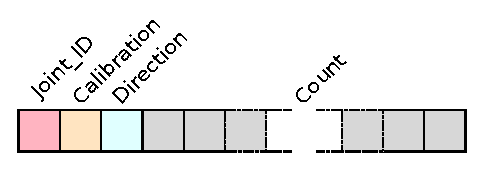
\includegraphics[width=.5\linewidth]{graphics/rf_packet}
	\caption[Structure of a packet used on the RF transmission between the joint boards and the controller board.]{Structure of a packet used on the RF transmission between the joint boards and the controller board. Bits 0-12 represent the current angular position, bit 13 represents the direction of motion, bit 14 represents the state of calibration and bit 15 represents the id of the joint.}
	\label{fig:rfpacket}
\end{figure}

With knowledge of the message size, it is possible to determine the theoretical maximum transmission rate.
The nRF24L01 module is capable of transmitting up to 2Mbps.
It uses Enhanced Shockburst, a protocol developed by Nordic Semiconductor specifically for their RF modules.
This protocol adds an overhead for each packet of 6 bytes, including a CRC check and an address, amongst a few other features.
Each packet is therefore $\approx$ 8 bytes with only 25\% of the packet being the intended payload.
This effectively limits the data rate to 0.5Mbps.
It is therefore possible to transmit a position at a rate of 31250Hz.
Since the two joints are communicating with the same module on the controller board, this frequency is halved resulting in 15625Hz.
Transmission at this frequency does entail a few problems, discussed in the following paragraphs.
\paragraph{nRF24L01 Mode Cycling}~\\ % (fold)
\label{par:nrf24l01_mode_cycling}
When transmitting at a rate of 15625Hz a message is to be sent every 64$\mu$s
According to the datasheet of the nRF24L01 it can be kept in transmit mode for no longer than 4ms, meaning that at the most 62 packets can be sent before cycling to standby-mode and back to TX-mode.
Before entering TX-mode a 130$\mu$s settling period is inferred.
This means that at least two packets are lost during this time.
The problem can be overcome by lowering the transmission frequency such that the time between packets is above 130$\mu$s.
6.25kHz transmission frequency would result in 160$\mu$s delay, enough time to cycle between the modes between each packet.
% paragraph nrf24l01_mode_cycling (end)
\paragraph{Air Collisions}~\\ % (fold)
\label{par:air_collisions}
There is a risk that two packets will collide if the joints transmit at the same time.
Due to uneven drift between the two microcontrollers on the joints it is unlikely that collisions will occur indefinitely, however even a few lost packets in a row can cause severe problems in the control of the pendulum.
The lowered transmission frequency alleviates this issue somewhat, but there is still a risk that multiple packets may be lost.
Air collisions could be overcome altogether by using the acknowledge feature in the Enhanced Shockburst protocol, this enables the module to resend a message if an ACK message has not been received within 250$\mu$s.
After 250$\mu$s however, the previous position is outdated and the new position should be sent rather than the lost position.
Additionally, the ACK message adds 15 bytes to the transmission of each packet, greatly lowering the possible throughput.
The nRF24L01 is capable of operating on different frequencies.
By adding a second receiver on the controller board the two joints can communicate on different frequencies, eliminating the risk of air collisions altogether.
This realisation was made after the controller board was produced and so the additional nRF24L01 has to be retrofitted on the board. 
% paragraph air_collisions (end)
\\~\\
In order to simplify communication between the joint boards and the controller board communcation will be one way only.
This allows the nRF24L01's on the controller board to stay in RX-mode, listening for new positions from the joints continuously.
The joint boards will, upon powering up, immediately start transmitting the packet mentioned in figure \ref{fig:rfpacket}.

\subsubsection{Requirements} % (fold)
\label{ssub:joint_software_requirements}

\subsection{Implementation} % (fold)
\label{sub:implementation}

\subsection{Verification} % (fold)
\label{sub:verification}
